% programming model
% ecall and ocall


Using the recently released Intel SGX SDK~\cite{sgxsdk}, we implmented the \tc
Server as an SGX-enabled application in C++. In the programming model supported by
the SDK, the body of an SGX-enabled application runs as an 
ordinary user-space application, while a relatively small piece of security-sensitive code runs in the isolated environment of the SGX enclave.

The enclave portion of an SGX-enabled application may be
viewed as a shared library exposing an API in the form of \emph{ecalls}
to be invoked by the untrusted application. Invocation of an ecall, however, transfers control to the 
enclave; the enclave code runs until it either terminates and explicitly releases control or some special event happens~\cite{sgxmanual}.
Again, as we assume SGX provides ideal isolation, the untrusted application cannot
observe or alter the execution of ecalls.

Enclave programs can make \emph{ocalls} to invoke functions defined outside of the enclave. An ocall triggers an exit from the enclave. Control is returned to the calling enclave code once the ocall completes. As ocalls execute outside the enclave, they must be treated by enclave code as untrusted. We emphasize that in \tc, only network functionality runs outside the enclave.

\begin{figure}[h]
    \centering
    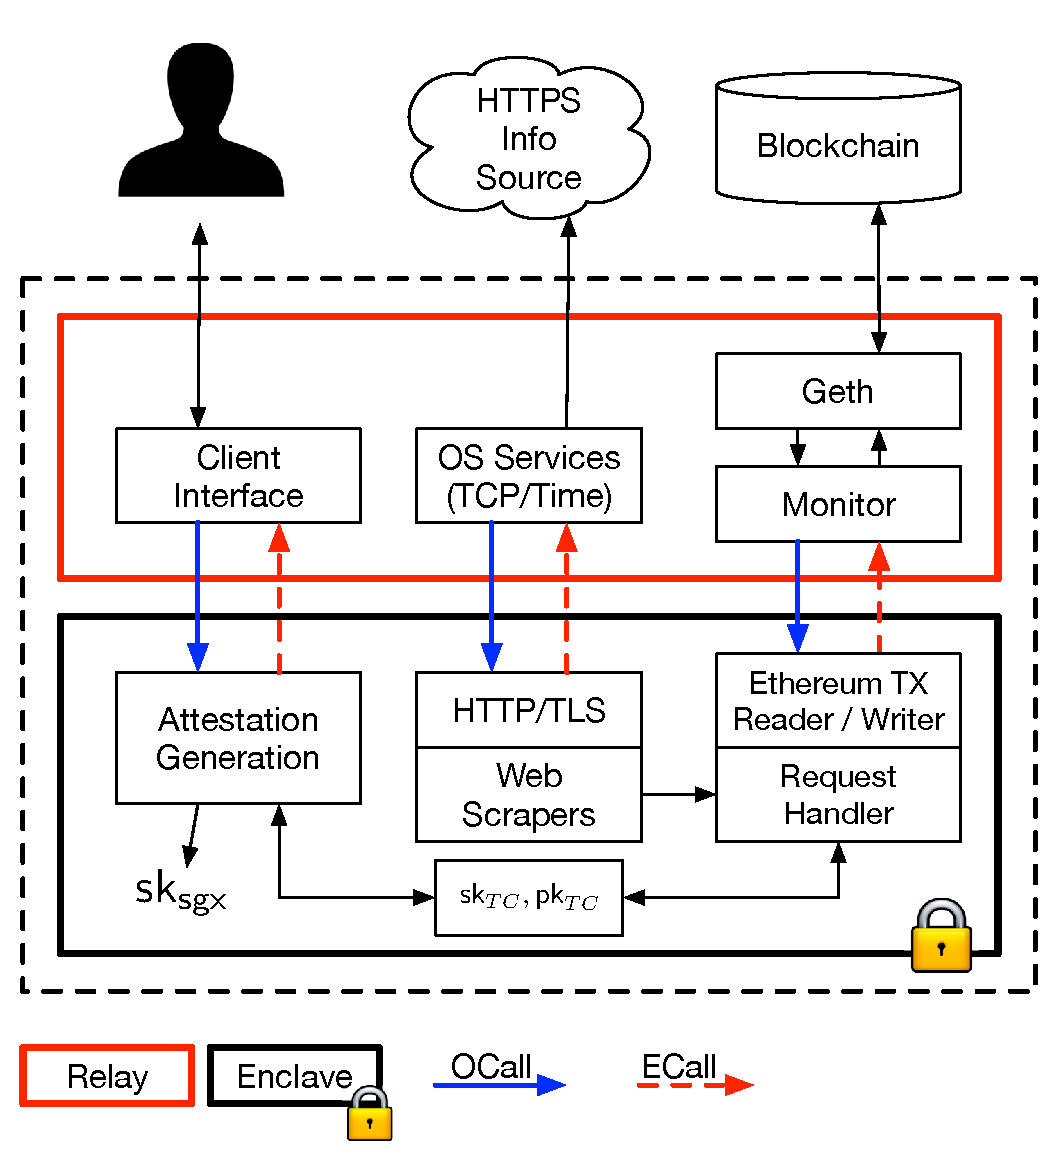
\includegraphics[width=0.45\textwidth]{figures/impl}
    \caption{Components of \tc Server}
    \label{fig:tcserver_impl}
\end{figure}

For \tc, we recall that Fig.~\ref{fig:engineprotocol} shows the enclave code $\engine$ and \ref{fig:relayprotocol} shows the \medname, the untrusted code in \tc. We now give details on the services they encompass and their interaction, summarized in Fig.~\ref{fig:tcserver_impl}, 

\paragraph{\bf The \encname.} There are three components to \engine: An HTTPS service, Web Scrapers, which interact with data sources, and a Request Handler, which services datagram requests. 

\vspace{2mm}

\noindent\emph{HTTPS Service.} We recall that the enclave does not have direct access to host network functionality. In \tc, we therefore partition HTTPS into a trusted layer, consisting of HTTP and TLS code, and an untrusted layer that provides low-layer network service in the form of TCP.  This arrangement allows the enclave to establish a secure channel with a web server: The enclave itself performs the TLS handshake with a target server and performs all cryptographic operations internally. The untrusted process acts as a network interface only. (Thus, if malicious, it can do no more harm than a generic network adversary.)  We ported a TLS library (mbedTLS) into the SGX environment as well as HTTP functionality minimized to meet the web-scraping requirements of \tc while keeping the TCB small. To verify certificates presented by remote servers, we hardcoded a collection of root CA certificates into the enclave code; in the first version of \tc, the root CAs are identical to those in Chrome.\ari{This seems reasonable to me, although there may be a better approach.}

\vspace{2mm}

\noindent\emph{Web Scrapers.} Extracting useful information from a given website is
implemented in a ad-hoc manner. For the purpose of demonstration, we implemented
three web scrapers as examples. \xxx[Fan]{Elaborate}.

\vspace{2mm}

\noindent\emph{Request Handler.} The Request Handler has two jobs: (1) Ingesting a datagram request by parsing 
it in the serialization format specified by Ethereum, decrypting it (if it's a private-datagram request), and dispatching its parameters to the right scraper; and (2) Returning the response to the request by generating an Ethereum
transaction containing the requested datagram (and parameters), serializing it as a blockchain transaction, and signing it using \skTC. We implemented the Ethereum ABI and RLP, which respectively
specify the serialization of arguments and transactions in Ethereum. 

\paragraph{Attestation Generation} \xxx[Fan]{Elaborate.}


\paragraph{The \medname.} The \medname encompasses three components: A Client Interface, which serves attestations and timestamps, OS services, including networking and time services, and a Blockchain Interface, as follows:

\vspace{2mm}

\noindent\emph{Client Interface.} As described in Section \ref{sec:architecture},
a client starts using \tc by requesting and verifying an attestation \att and checking the correctness of the clock in the \tc enclave using a fresh timestamp.
The Client Interface caches \att upon initialization of \engine. When it receives a web request from a client for an attestation,
it issues an ecall to the enclave to obtain a
Unix timestamp signed under \pkTC, which it returns to the client along with \att. The client can check the timestamp using any trustworthy time service and verify \att 
using the Intel Attestation Service (IAS)~\cite{}. 

\vspace{2mm}

\noindent\emph{OS services.} The \encname relies on the \medname to access networking and 
time services \ari{What time services?} provided by the OS and implemented as ocalls.

\vspace{2mm}

\noindent\emph{Blockchain Interface.} The \medname's Blockchain Interface monitors the
blockchain for incoming requests and places transactions on the blockchain in order to
deliver datagrams. The Blockchain Interface incorporates an 
official Ethereum client, Geth~\cite{geth}. This Geth client is configured with a JSON RPC server through which the
\medname can communicate with the blockchain indirectly via RPC calls. For example, to insert a signed transaction, the \medname can simply call
\texttt{eth\_sendRawTransaction} with the byte array of the serialized
transaction. We emphasize that as the enclave holds \skTC, transactions must be signed within the enclave.


